\chapter{Developing the Observation Strategy for GOTO}
\label{chap:strategy}
\chaptoc{}

% ########################################

\newpage
\section{Introduction}
\label{sec:strategy_intro}
\begin{colsection}

% ~~~~~~~~~~~~~~~~~~~~

\begin{colsection}

In this chapter I outline my work developing the observing strategy for the GOTO prototype telescope.
\rtxt{Thanks to Darren and Evert <blah><blah><blah>}

\end{colsection}

% ~~~~~~~~~~~~~~~~~~~~

\subsection{GOTO as a survey telescope}
\label{sec:survey_telescope}
% normal mode of operation
% compare to other survey telescopes - ASSASSIN [sic], ZTF
\begin{colsection}

WIP

\end{colsection}

% ~~~~~~~~~~~~~~~~~~~~

\subsection{GOTO as a follow-up telescope}
\label{sec:followup_telescope}
\begin{colsection}

WIP

\end{colsection}

% ~~~~~~~~~~~~~~~~~~~~

\end{colsection}

% ########################################

\newpage
\section{Tiling the sky}
\label{sec:tiling}
\begin{colsection}

% ~~~~~~~~~~~~~~~~~~~~

\begin{colsection}

WIP

\end{colsection}

% ~~~~~~~~~~~~~~~~~~~~

\subsection{GOTO-tile}
\label{sec:gototile}
% different ways to make grids
\begin{colsection}

GOTO-tile is a \proglang{Python} module (\pkg{gototile} \rtxt{footnote url?}) created for the \gls{goto} project to contain all the functions and frameworks related to tiling the sky. It was originally developed by Darren White as a way to process \gls{ligo} \gls{gw} skymaps for \gls{goto}, and then maintained by Evert Rol who rearranged it into a module usable for some other telescopes including SuperWASP on La Palma and a proposed southern GOTO node. My contributions to the module have been more fundamental: reworking the foundations to improve how grids are defined and sky maps are applied to them, as well as adding different ways to create skymaps.

% ---------
\subsubsection{Sky grids}

The core of GOTO-tile as it now exists is the \code{SkyGrid} class. This is used to define a sky grid, a collection of `tiles' defined as points on the celestial sphere. These tiles are aligned to the celestial right ascension/declination coordinates, and are designed to create a base framework for observations to be mapped to.

The most important parameter required when defining a sky grid is the field of view of the telescope, which is taken as the size of the tiles that make up the grid. This is defined by giving a width and height value in degrees, meaning the tiles can only be square or rectangular. This is typically fine for the \gls{goto} array, although there was a period when having three \glspl{ut} in an `L'-shape was considered. This was abandoned due mainly to the complexity of tiling the grid based on abstract shapes.

The second parameter required to define a sky grid is the desired overlap between the tiles. This is given as a value between zero and one in both the right ascension and declination directions, with zero meaning no overlap and one meaning all the tiles are completely overlapping (as this would lead to infinite tiles being created in practice the overlap is restricted to no more than $0.9$). This is used to define the spacing between the tile centrers, although exactly how depends on the algorithm used.

As GOTO-tile has been developed the algorithm used to define tile centres has evolved and improved. I wrote the latest algorithm, called \code{minverlap}, to


\begin{figure}[pt]
\begin{center}
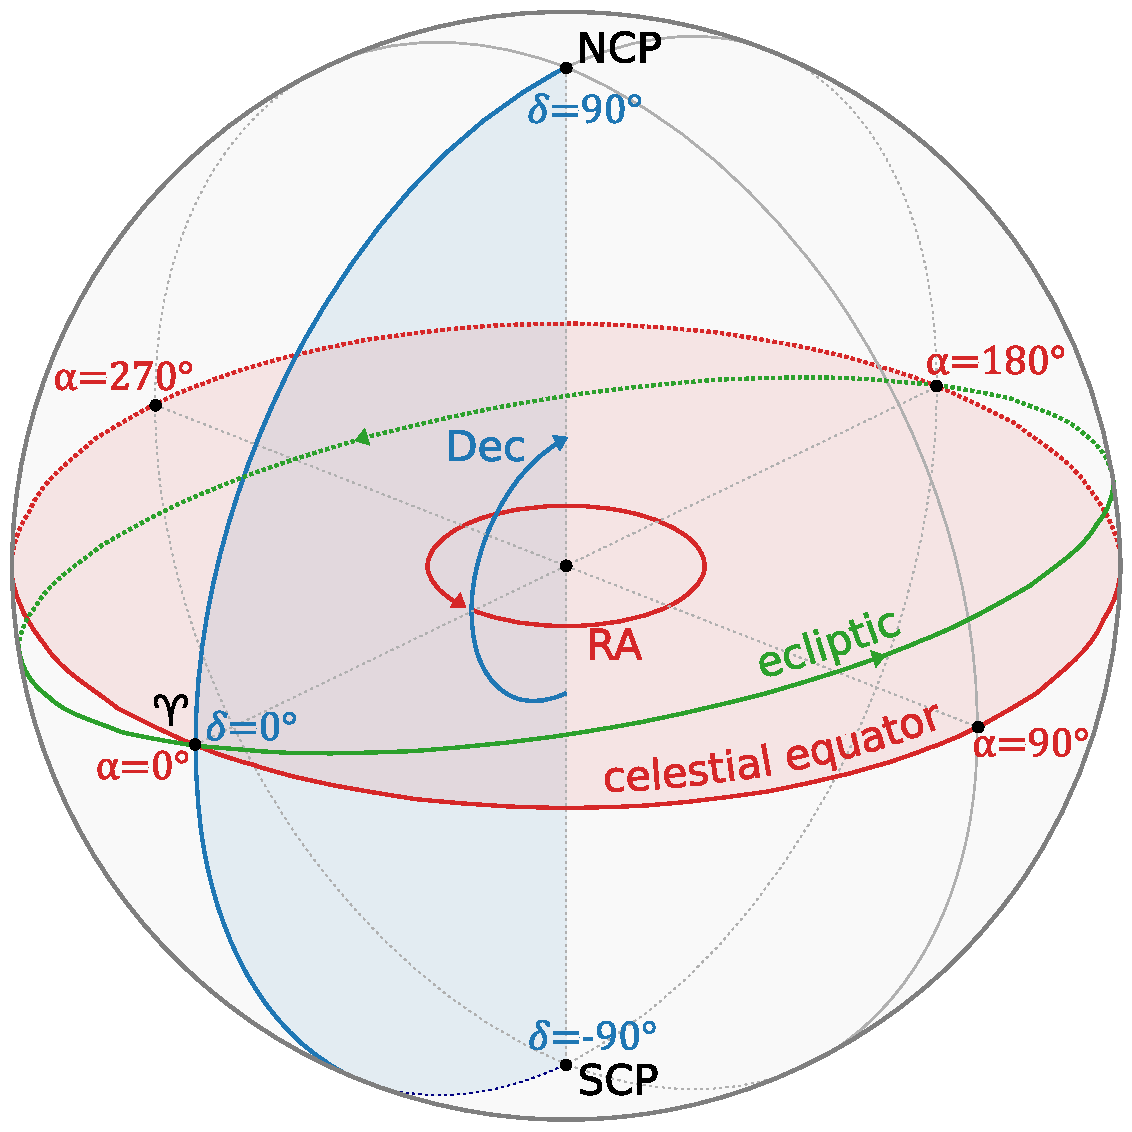
\includegraphics[width=\linewidth]{images/globe1.pdf}
\end{center}
\caption[The celestial sphere]{The celestial sphere. The celestial equator is marked in \textcolor{red}{red}, the vernal equinox (where the ecliptic (not shown) crosses the equator) is marked with the symbol \Aries{} and the meridian that intercepts the vernal equinox is marked in \textcolor{blue}{blue}. The northern and southern celestial poles are marked as NCP and SCP respectively. The definition of the equatorial coordinate system is shown: declination (Dec, $\delta$) is defined as the angle from the equator, ranging from \SI{-90}{\degree} at the SCP to \SI{90}{\degree} at the NCP, and right ascension (RA, $\alpha$) is defined as angle east from the vernal equinox between \SI{0}{\degree} and \SI{360}{\degree}.
}
\label{fig:sphere}
\end{figure}

\begin{figure}[pt]
\begin{center}
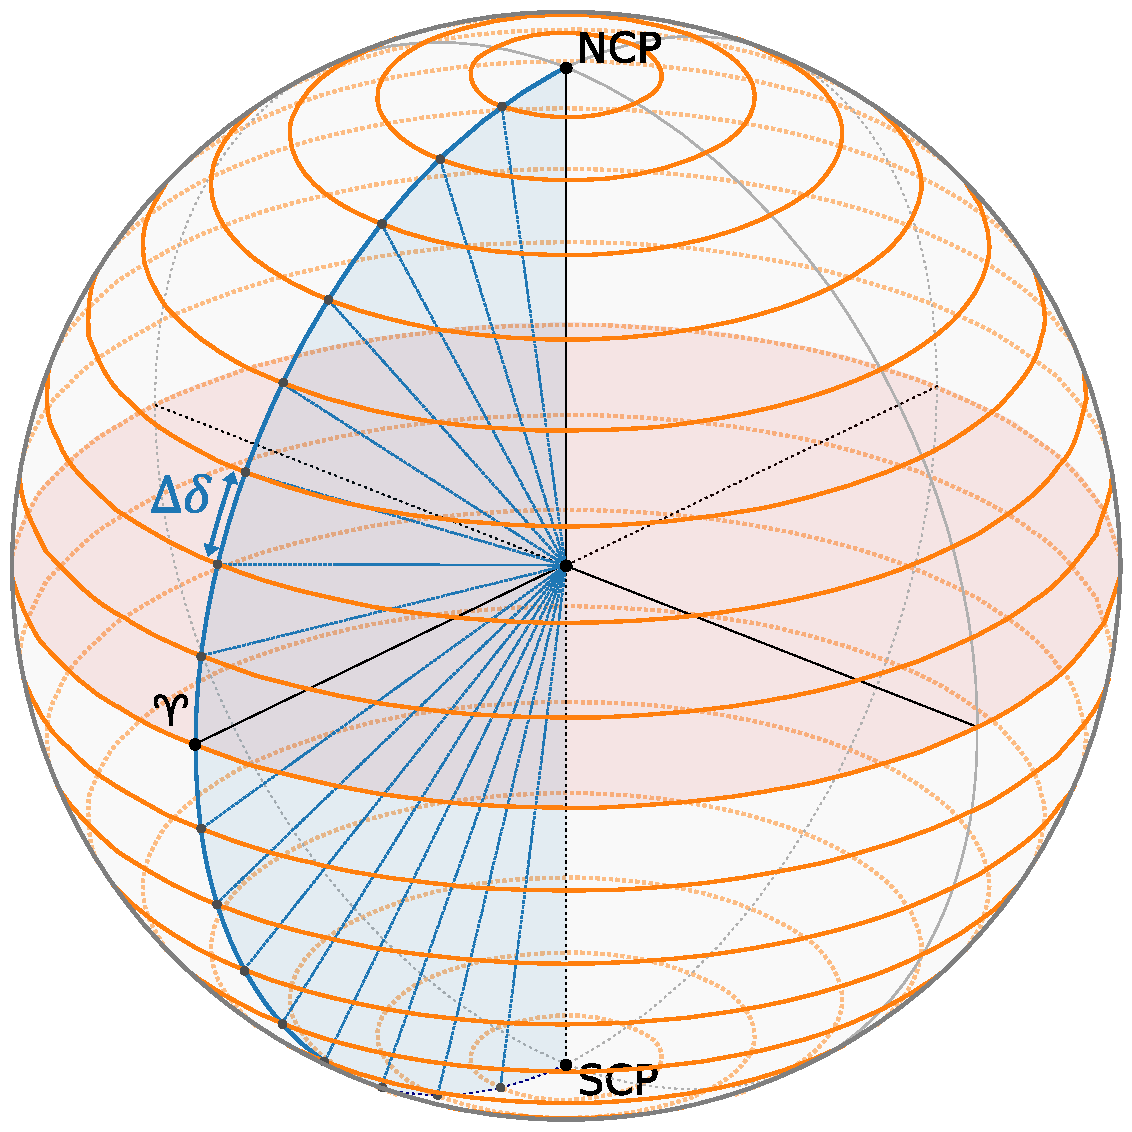
\includegraphics[width=\linewidth]{images/globe2.pdf}
\end{center}
\caption[Defining declination strips]{The first stage when creating a sky grid is defining the declination strips. This is done by dividing the full range of declination (\SI{-90}{\degree} to \SI{90}{\degree}) equally by a constant spacing value $\Delta\delta$. In this example $\Delta\delta =$ \SI{10}{\degree}, and so strips are defined at $\delta=$ \SI{0}{\degree}, \SI{10}{\degree}, \SI{20}{\degree} etc\ldots, and mirrored in the southern hemisphere. There is always a strip with $\delta=0$. Exactly how the strips are defined when $\Delta\delta$ is not an integer factor of \SI{90}{\degree} depends on the algorithm used, in this case using the ``minverlap'' algorithm the strips range from \SI{-90}{\degree} to \SI{90}{\degree} and include a ``strip'' at the poles which will contain single tile (as shown in Figure~\ref{fig:tiledsphere}).
}
\label{fig:deltadelta}
\end{figure}

\begin{figure}[pt]
\begin{center}
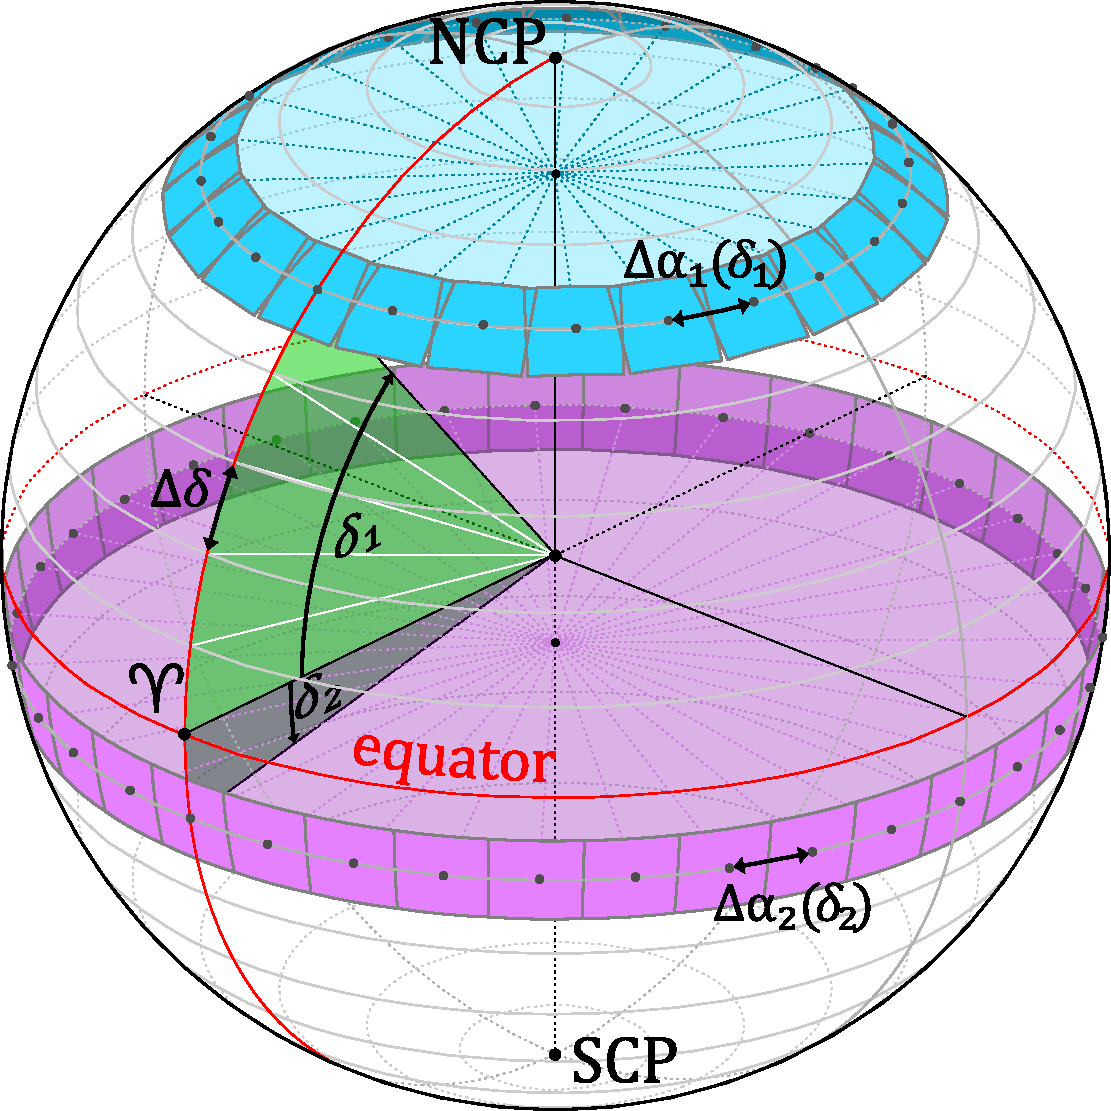
\includegraphics[width=\linewidth]{images/globe3.pdf}
\end{center}
\caption[Defining the spacing between tiles]{After the declination strips are defined (see Figure~\ref{fig:deltadelta}) for each strip tile centres are defined with a set spacing $\Delta\alpha(\delta)$. Unlike $\Delta\delta$, which is fixed across the sphere, $\Delta\alpha$ varies as a function of declination meaning strips closer to the poles will contain fewer tiles. Two examples of defining tiles are shown above, one at declination $\delta_1$ (\SI{50}{\degree}, in \textcolor{cyan}{light blue}) in the northern hemisphere and another at $\delta_2$ (\SI{-10}{\degree}, in \textcolor{Plum}{purple}) in the southern hemisphere. The results of the ``minverlap'' algorithm are shown, previous algorithms had different ways of defining $\Delta\alpha$ that would have resulted in different spacings.
}
\label{fig:deltaalpha}
\end{figure}

\begin{figure}[pt]
\begin{center}
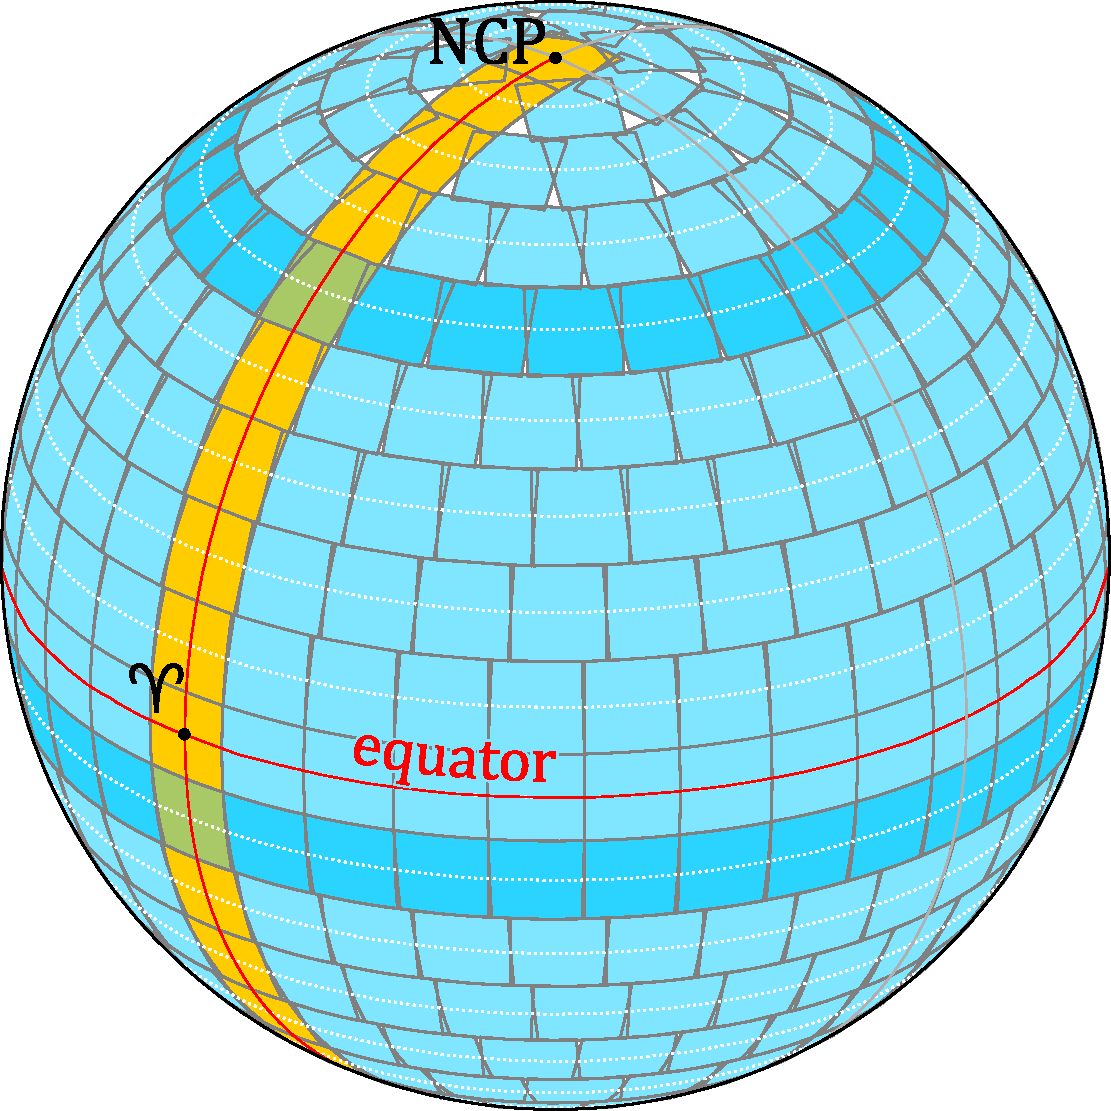
\includegraphics[width=\linewidth]{images/globe4.pdf}
\end{center}
\caption[A fully tiled sphere]{Once every declination strip is complete the full grid is defined, as shown above. The same two strips are shown in \textcolor{cyan}{light blue} and \textcolor{Plum}{purple} as in Figure~\ref{fig:deltaalpha}. Due to each strip starting the tile spacing at RA$=0$, there is a fully aligned column of tiles along the vernal equinox, shown in \textcolor{orange}{yellow}. The grid in these examples was defined using the ``minverlap'' algorithm, with each tile having a field of view of \SI{10}{\degree} $\times$ \SI{10}{\degree} and the overlap was set to zero for clarity (note this leads to gaps between tiles towards the poles). In this case the full grid contains 424 tiles.
\\
}
\label{fig:tiledsphere}
\end{figure}









\end{colsection}

% ~~~~~~~~~~~~~~~~~~~~

\subsection{The all-sky grid}
\label{sec:survey}
\begin{colsection}

WIP

\end{colsection}

% ~~~~~~~~~~~~~~~~~~~~

\subsection{Advantages and disadvantages of a fixed grid}
\label{sec:fixed_grid}
\begin{colsection}

WIP

\end{colsection}

% ~~~~~~~~~~~~~~~~~~~~

\subsection{Observing on the grid}
\label{sec:grid_observing}
\begin{colsection}

WIP

\end{colsection}

% ~~~~~~~~~~~~~~~~~~~~

\end{colsection}

% ########################################

\newpage
\section{Automated alert follow-up}
\label{sec:followup}
\begin{colsection}

% ~~~~~~~~~~~~~~~~~~~~

\begin{colsection}

WIP

\end{colsection}

% ~~~~~~~~~~~~~~~~~~~~

\subsection{Alert processing}
\label{sec:alerts}
\begin{colsection}

WIP

\end{colsection}

% ~~~~~~~~~~~~~~~~~~~~

\subsection{Scheduler simulations}
\label{sec:simulations}
\begin{colsection}

WIP

\end{colsection}

% ~~~~~~~~~~~~~~~~~~~~

\subsection{Gravitational wave observations}
\label{sec:gw_followup}
\begin{colsection}

WIP

\end{colsection}

% ~~~~~~~~~~~~~~~~~~~~

\subsection{Other transient follow-up}
\label{sec:other_followup}
\begin{colsection}

WIP

\end{colsection}

% ~~~~~~~~~~~~~~~~~~~~

\end{colsection}

% ########################################
